\documentclass{beamer}
% \usepackage[utf8]{inputenc}
\usepackage[T1]{fontenc}
\usetheme{CambridgeUS}
\useoutertheme{miniframes}
\usecolortheme{dove}
\usefonttheme{serif}
\beamertemplatenavigationsymbolsempty
\usepackage{lmodern}
\usepackage[scale=2]{ccicons}
\usepackage{tikz}

\setbeamertemplate{background}{\tikz[overlay,remember picture]\node[opacity=0.07]at (current page.center){
\includegraphics[width=8cm]{images/logo-PW.png}};}

\defbeamertemplate{headline}{pwtemplate}{
    \leavevmode%
    \hbox{%
        \begin{beamercolorbox}[wd=\paperwidth,ht=2.25ex,dp=1ex,right]{title in head/foot}%
            \usebeamerfont{title in head/foot}\insertframenumber/\inserttotalframenumber\hspace*{2em}
        \end{beamercolorbox}}%
    \vskip0pt% 
}

\defbeamertemplate{footline}{pwtemplate}{%
    \leavevmode
    \setbeamercolor{lfooterbox}{bg=gray!10}
    \begin{beamercolorbox}[wd=.33\paperwidth,ht=7pt,dp=4pt,center]{lfooterbox}%
        \usebeamerfont{author in head/foot}\insertshortauthor
    \end{beamercolorbox}%
    \setbeamercolor{cfooterbox}{bg=gray!20}
    \begin{beamercolorbox}[wd=.34\paperwidth,ht=7pt,dp=4pt,center]{cfooterbox}%
        \usebeamerfont{date in head/foot}\insertshorttitle
    \end{beamercolorbox}%
    \setbeamercolor{rfooterbox}{bg=gray!10}
    \begin{beamercolorbox}[wd=.33\paperwidth,ht=7pt,dp=4pt,center]{rfooterbox}%
        \usebeamerfont{title in head/foot}\insertshortinstitute
    \end{beamercolorbox}
}


\usepackage[english]{babel}
% \usepackage[english, polish]{babel}

\usepackage{listings}
\lstset{basicstyle=\ttfamily\footnotesize,breaklines=true}
\usepackage{siunitx}
\usepackage{pifont}
\usepackage{amsmath,amssymb,amsfonts}
\usepackage{graphicx}
\usepackage[export]{adjustbox}
\usepackage{float}
\usepackage{xcolor}
\usepackage{setspace}

\newcommand{\todo}[1]{\textcolor{red}{TODO: #1}}

\newcommand{\imagesource}[1]{
    \begin{spacing}{0.5}
        \texttt{\textit{ \tiny{source: #1}}}
    \end{spacing}
}

\newenvironment{columnframe}[1]{
    \begin{frame}[environment=columnframe,fragile]{#1}
        \begin{columns}
            }{
        \end{columns}
    \end{frame}
}




\title[STS]{Silicon Tracking System}
    \subtitle{\textit{at the CBM experiment}}
\author[T. Fic]{Tobiasz Fic}
\institute[WUT]{Warsaw University of Technology}
\date{4 June 2024}

\begin{document}

\setbeamertemplate{headline}{}
\setbeamertemplate{footline}{}

\setbeamertemplate{background}{\tikz[overlay,remember picture]\node[opacity=0.07]at (current page.center){
\includegraphics[width=8cm]{images/logo-PW.png}};}
\begin{frame}
    \maketitle
\end{frame}
\setbeamertemplate{background}{}

\setbeamertemplate{headline}[pwtemplate]
\setbeamertemplate{footline}[pwtemplate]

\begin{columnframe}{GSI and FAIR}
    \begin{column}{0.5\textwidth}
        \begin{figure}
            \centering
            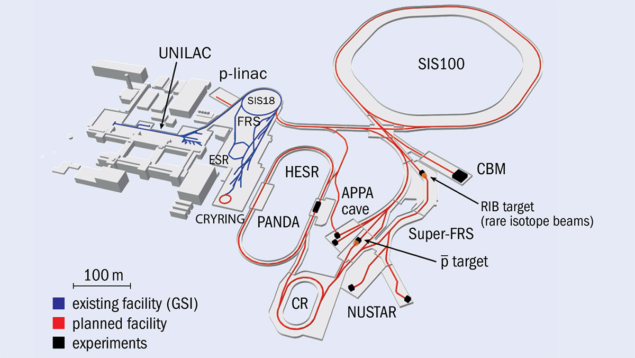
\includegraphics[width=\textwidth, frame]{images/fair_sis100_diagram.jpg}
        \end{figure}
    \end{column}
    \begin{column}{0.5\textwidth}
        \begin{itemize}
            \item The Facility for Antiproton and Ion Research (FAIR) is currently
                  under construction at the GSI (Gesellschaft fur SchwerIonenforschung)
                  Helmholtz Centre for Heavy Ion Research in Darmstadt, Germany
        \end{itemize}
    \end{column}
\end{columnframe}

\begin{columnframe}{The CBM Experiment}
    \begin{column}{0.5\textwidth}
        \begin{itemize}
            \item The CBM experiment aims to study the properties of nuclear matter at high baryon densities
            \item The energy range is between 2 and 5 GeV (beam momentum up to 12 AGeV/c)
                  (SIS100 accelerator at FAIR)
            \item The interaction rate is up to 10 MHz
            \item The planned start date is 2027
        \end{itemize}
    \end{column}
    \begin{column}{0.5\textwidth}
        \begin{figure}
            \centering
            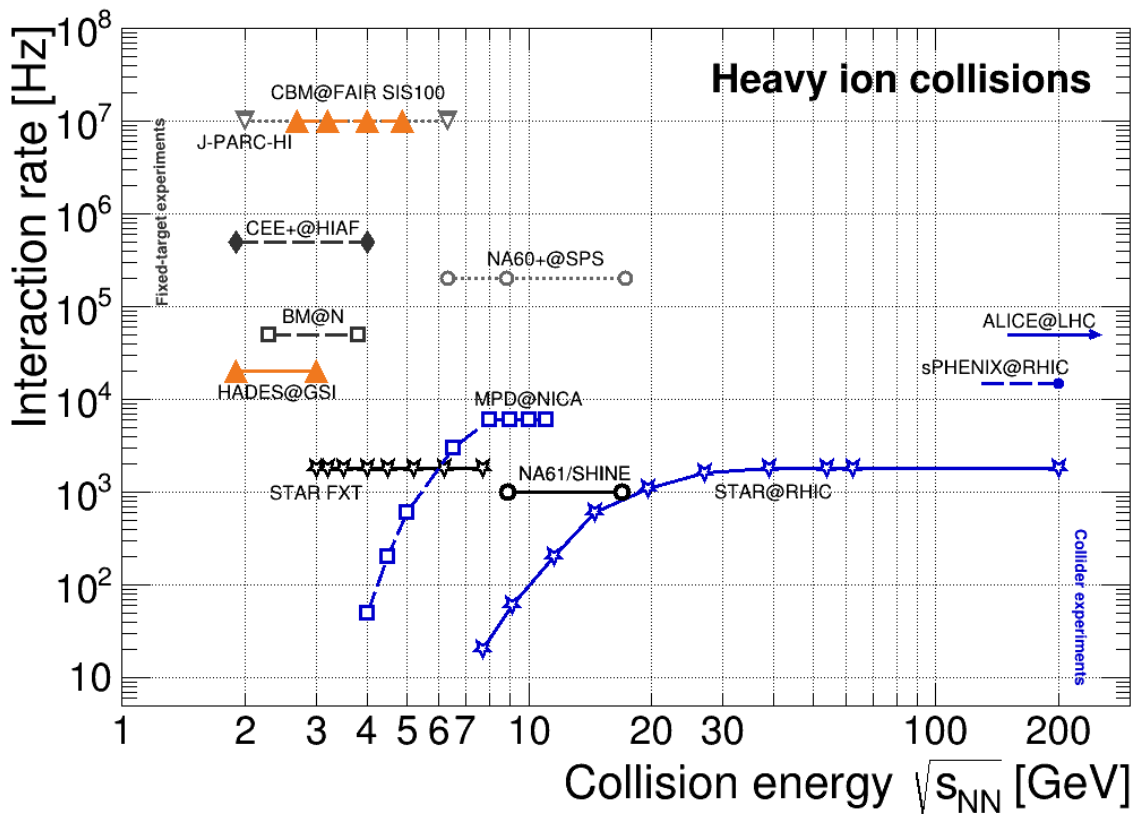
\includegraphics[width=\textwidth, frame]{images/galatyuk_map_of_experiments.png}
        \end{figure}
    \end{column}
\end{columnframe}

\begin{frame}{The CBM experiment detector setup}
    \begin{figure}
        \centering
        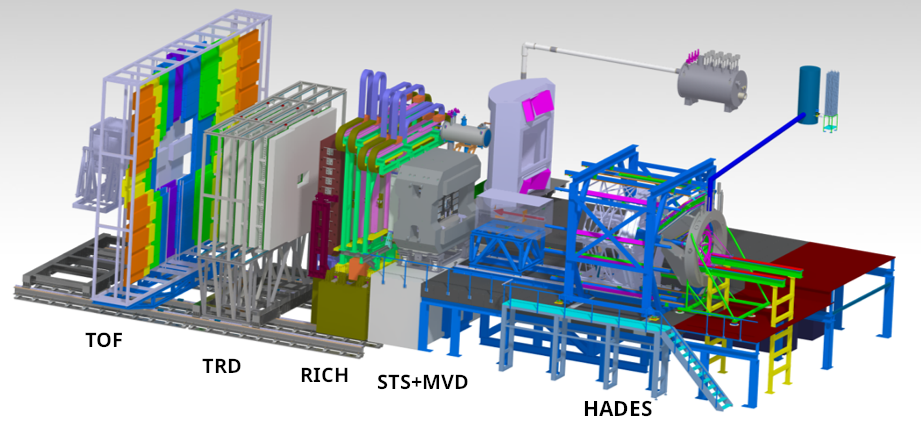
\includegraphics[width=\textwidth, frame]{images/CBM_HADES_new_setup.png}
    \end{figure}
\end{frame}

\begin{columnframe}{Silicon Tracking System - goals}
    \begin{column}{0.5\textwidth}
        \begin{figure}
            \centering
            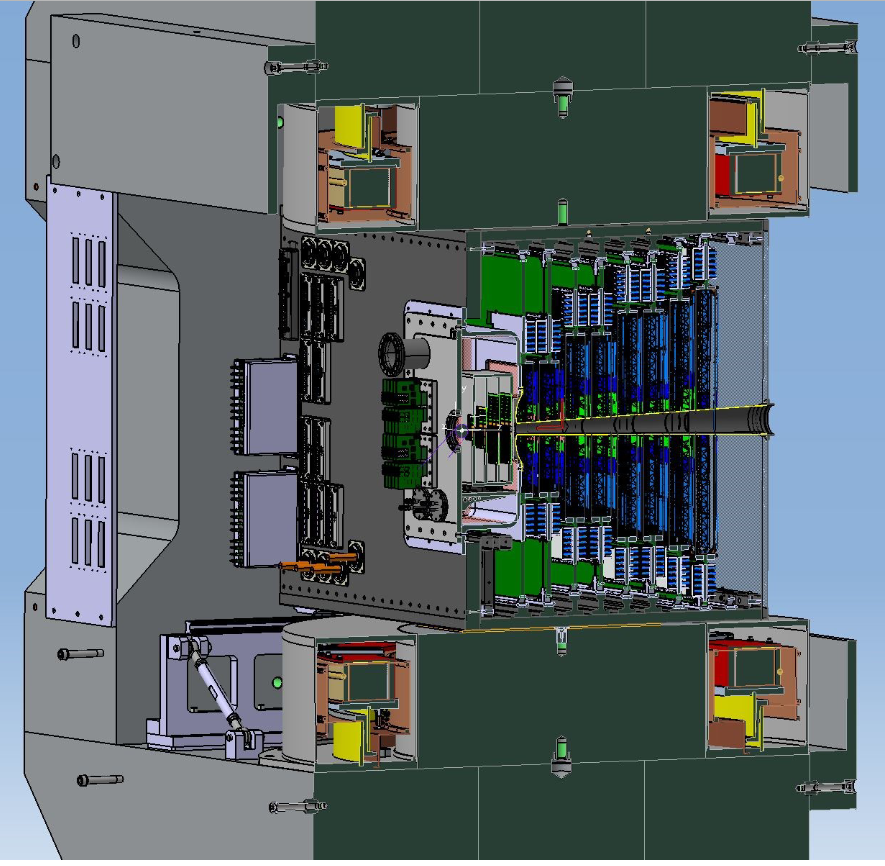
\includegraphics[width=0.6\textwidth, frame]{images/sts_render.png}
        \end{figure}
    \end{column}
    \begin{column}{0.5\textwidth}
        \begin{itemize}
            \item STS is the main tracking system at CBM.
            \item Measuring $dE/dx$ values at many stations
            \item Locked in a large magnet, so tracks of charged particles are curved
        \end{itemize}
    \end{column}
\end{columnframe}

\begin{columnframe}{Silicon Tracking System - overview}
    \begin{column}{0.5\textwidth}
        \begin{itemize}
            \item spatial resolution $\approx$ $25\mu m$
            \item time-stamp resolution $\approx$ $5ns$
            \item power dissipation: $~40kW$ ($CO_2$ cooling - sensors at $T\approx -5\si{\celsius}$)
            \item momentum resolution: $dp/p \approx 1.8\%$ (at $p > 1 GeV/c$, 1 Tm uniform field)
            \item self-triggering electronics
        \end{itemize}
    \end{column}
    \begin{column}{0.5\textwidth}
        \begin{figure}
            \centering
            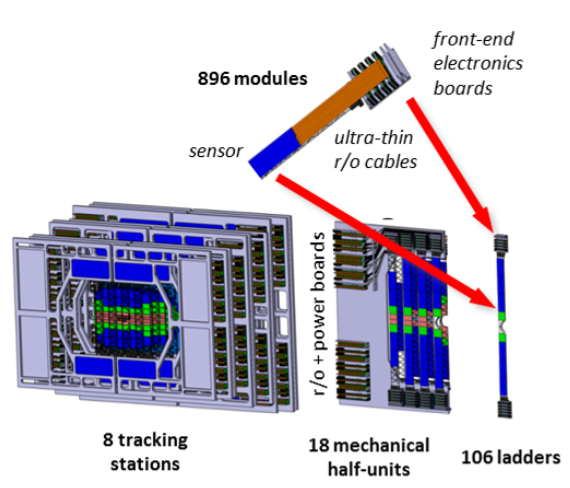
\includegraphics[width=0.9\textwidth, frame]{images/sts_integration_model.png}
        \end{figure}
    \end{column}
\end{columnframe}
\begin{columnframe}{STS - Dimensions}
    \begin{column}{0.5\textwidth}
        \begin{figure}
            \centering
            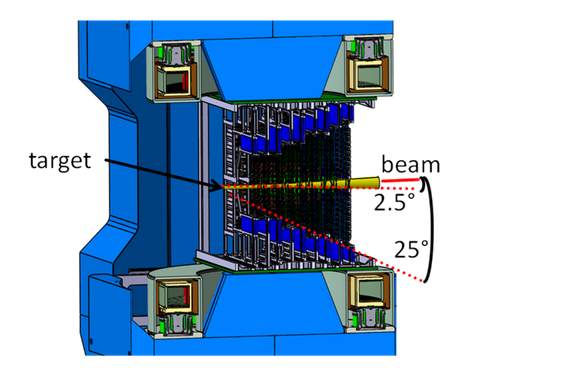
\includegraphics[width=0.6\textwidth, frame]{images/sts_dimensions.png}
        \end{figure}
    \end{column}
    \begin{column}{0.5\textwidth}
        \begin{itemize}
            \item 1.4x2x1.1m
            \item 8 tracking stations: volume $2m^3$, area $4m^2$
            \item 896 double-sided micro-strip silicon sensors
        \end{itemize}
    \end{column}
\end{columnframe}

\begin{columnframe}{STS - the Magnet}
    \begin{column}{0.5\textwidth}
        \begin{itemize}
            \item Working gap is 1.4x2.5m
            \item Weighs roughly 150 tons
            \item Cooled with helium
        \end{itemize}
    \end{column}
    \begin{column}{0.5\textwidth}
        \begin{figure}
            \centering
            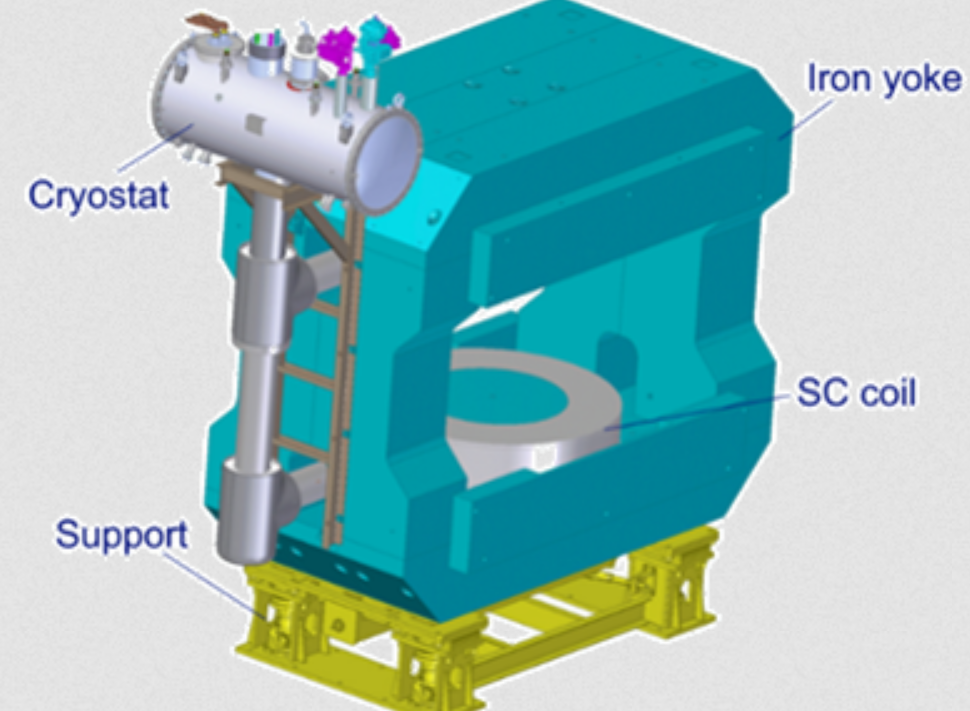
\includegraphics[width=0.8\textwidth, frame]{images/sts_magnet.png}
        \end{figure}
    \end{column}
\end{columnframe}

\begin{columnframe}{STS - silicon sensors}
    \begin{column}{0.5\textwidth}
        \begin{figure}
            \centering
            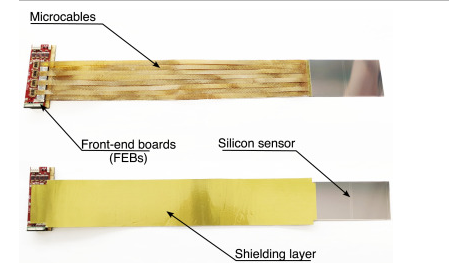
\includegraphics[width=\textwidth, frame]{images/sts_silicon_sensor.png}
            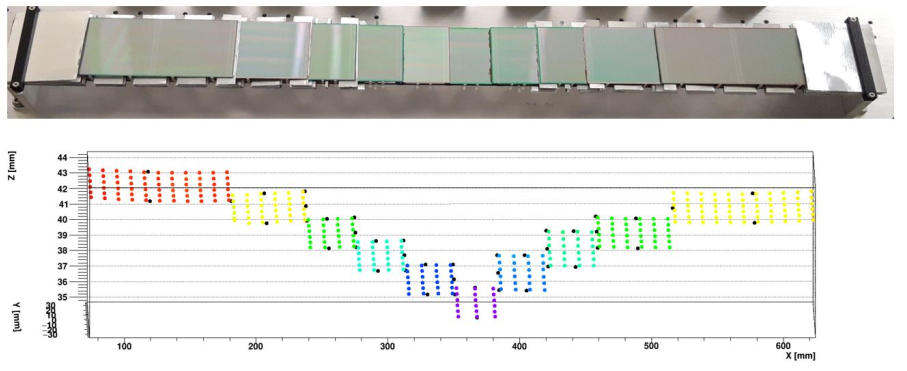
\includegraphics[width=\textwidth]{images/sts_strips.png}
        \end{figure}
    \end{column}
    \begin{column}{0.5\textwidth}
        \begin{itemize}
            \item Thin silicon strips pick up disturbances in the electric field
                  caused by charged particles travelling through the detector
            \item The signal from the strips is passed to the electronics via aluminum
                  microcables (128 per sensor, 896 sensors in total)
                  (in essence a voltage is probed)
            \item What if a cable breaks?
        \end{itemize}
    \end{column}
\end{columnframe}
\begin{columnframe}{STS - calibration}
    \begin{column}{0.5\textwidth}
        \begin{itemize}
            \item The response of each silicon sensor should be normalized.
            \item In addition, the electronics must be calibrated both for
                  gain (aplifiers) and time.
            \item Noise performance is evaluated for the sensors and microcables
                  separately.
            \item At the interaction rate of 10 MHz, capacitance of cables and sensors
                  starts to pose an issue.
        \end{itemize}
    \end{column}
    \begin{column}{0.5\textwidth}
        \begin{figure}
            \centering
            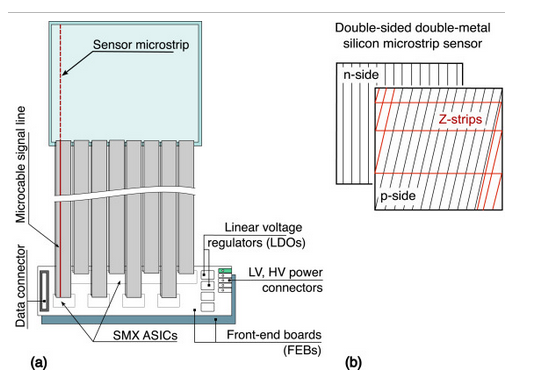
\includegraphics[width=\textwidth]{images/sts_microstrip_silicon.png}
            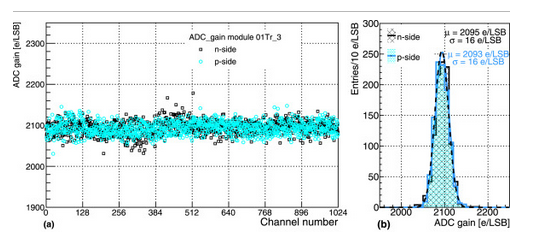
\includegraphics[width=\textwidth]{images/sts_calibration_plots.png}
        \end{figure}
    \end{column}
\end{columnframe}

\begin{columnframe}{STS - reconstruction}
    \begin{column}{0.5\textwidth}
        \begin{figure}
            \centering
            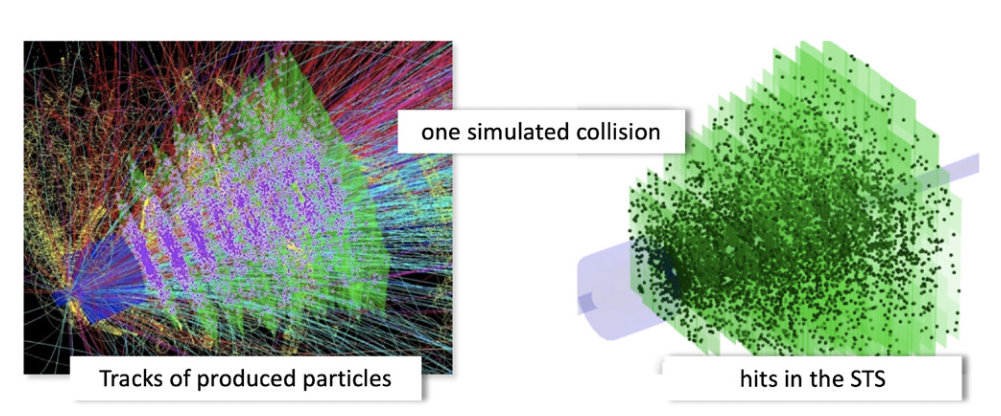
\includegraphics[width=0.9\textwidth, frame]{images/sts_reco.png}
        \end{figure}
    \end{column}
    \begin{column}{0.5\textwidth}
        \begin{itemize}
            \item The CBMRoot framework is used for the reconstruction
            \item The software is written in C++, currently using data
                  from GEANT4 simulations
            \item The plan is to be able to do reconstruction in real-time (online) using FPGAs
            \item The (simulated) tracking efficiency is $95\%$
        \end{itemize}
    \end{column}
\end{columnframe}

\begin{columnframe}{STS - current state (mCBM)}
    \begin{column}{0.5\textwidth}
        \begin{itemize}
            \item Since SIS100 is not yet operational, the mCBM (miniCBM) experiment is being
                  conducted at the SIS18 accelerator
            \item The magnet has not yet been delivered (due to trading sanctions with Russia),
                  so the STS tests are being conducted without momentum measurement
        \end{itemize}
    \end{column}
    \begin{column}{0.5\textwidth}
        \begin{figure}
            \centering
            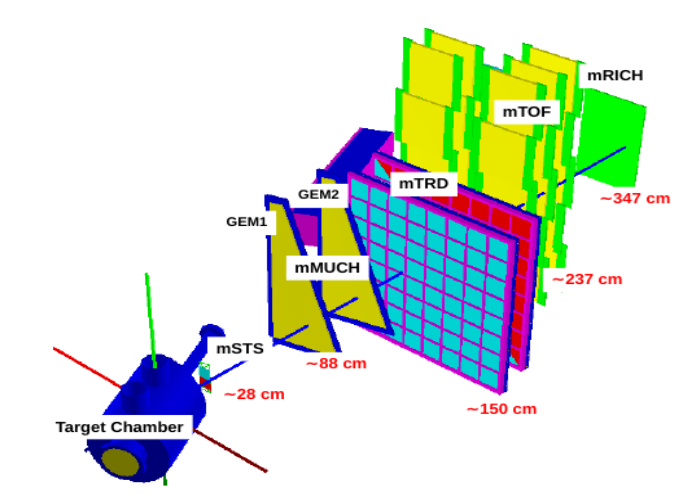
\includegraphics[width=0.7\textwidth, frame]{images/mCBM_render.png}
        \end{figure}
    \end{column}
\end{columnframe}


\begin{columnframe}{Outlook}
    \begin{column}{0.5\textwidth}
        \begin{figure}
            \centering
            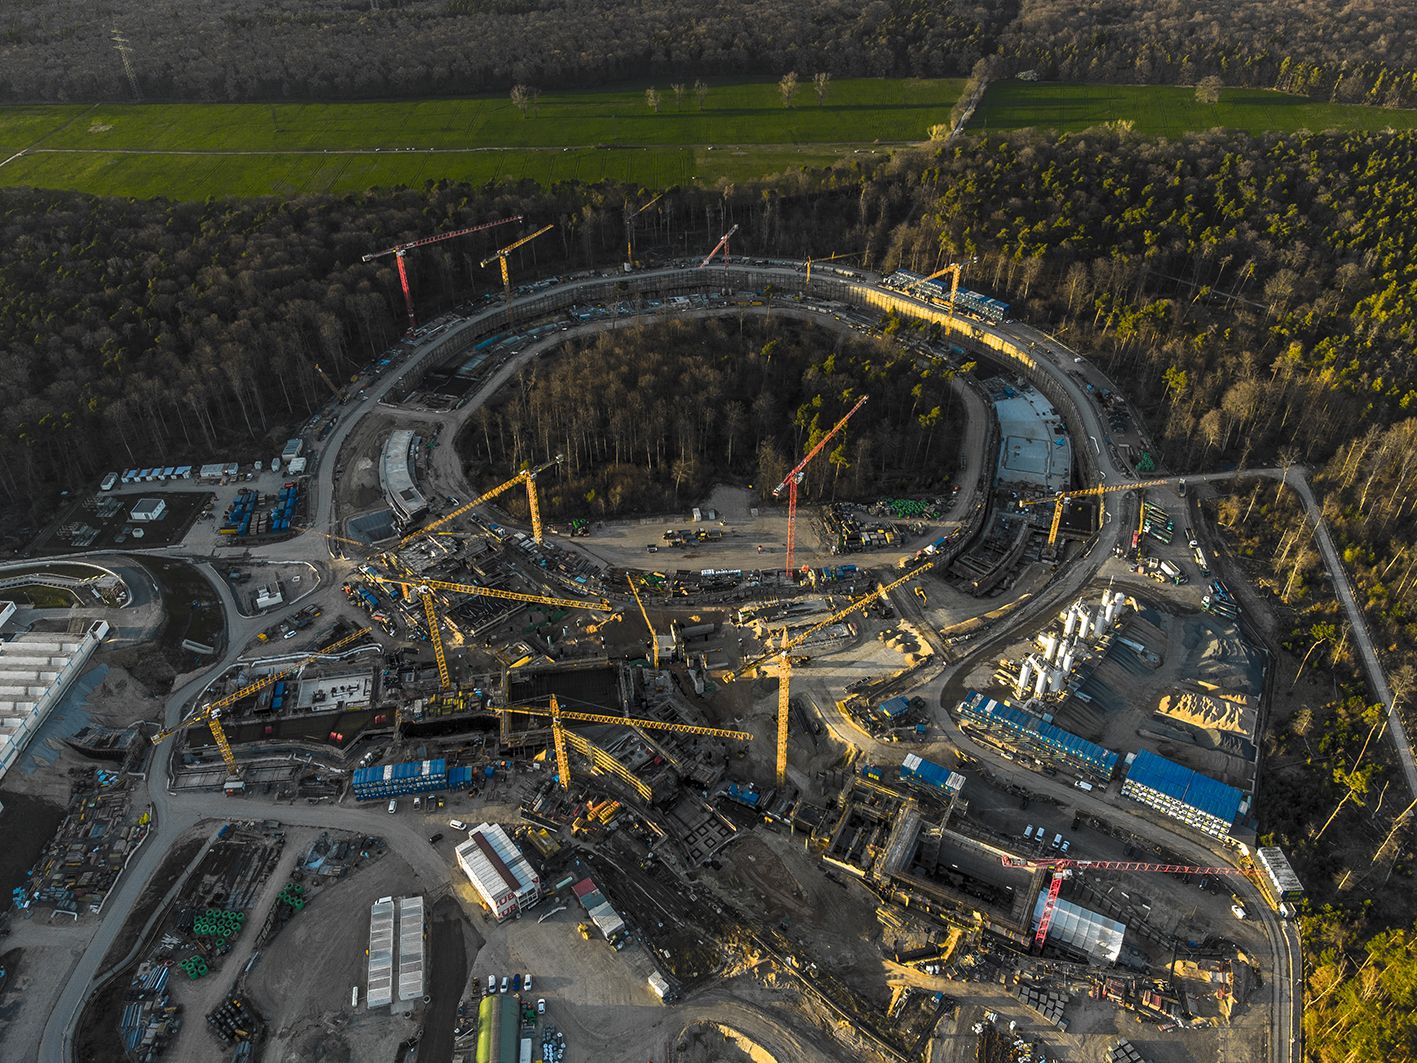
\includegraphics[width=0.7\textwidth, frame]{images/sis100_construction_site.jpg}
        \end{figure}
    \end{column}
    \begin{column}{0.5\textwidth}
        \begin{itemize}
            \item The STS detector is on track to be finished by the time SIS-100 is operational
            \item The aforementioned tracking software is being tested on simulations
        \end{itemize}
    \end{column}
\end{columnframe}

\begin{frame}
    \centering
    \Large{Questions?}
\end{frame}

\setbeamertemplate{headline}{}
\setbeamertemplate{footline}{}
\begin{frame}{}
    \centering
    \Large{Thank you for your attention}
\end{frame}

\end{document}